% This should be \input first thing after \begin{document}



\pagestyle{titlepage}

\begin{center}
   {\Huge  DUNE Computing Consortium}  %Yes, I know title and subtitle are reversed!

  \vspace{5mm}

  {\Huge  Conceptual Design Report}  

  \vspace{10mm}

 

\titleextra  %--- add back in if you want a picture here

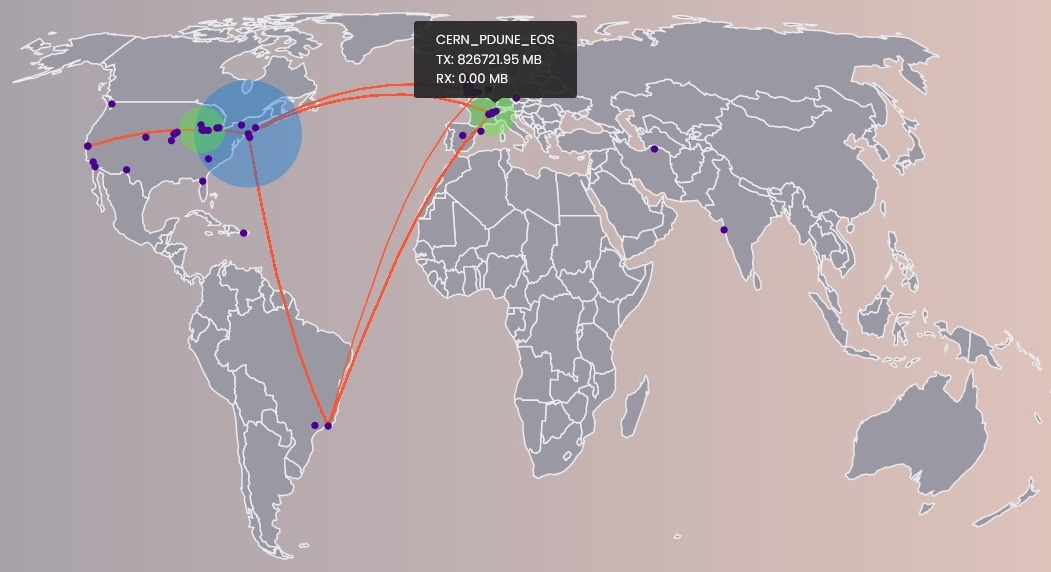
\includegraphics[width=\textwidth]{graphics/dune-firstVersionNotBad-show.jpg}

  \vspace{10mm}
  \today
    \vspace{15mm}
    
    {\large{The DUNE Collaboration}}
\end{center}

\cleardoublepage
\vspace*{16cm} 
  {\small  This document was prepared by the DUNE collaboration using the resources of the Fermi National Accelerator Laboratory (Fermilab), a U.S. Department of Energy, Office of Science, HEP User Facility. Fermilab is managed by Fermi Research Alliance, LLC (FRA), acting under Contract No. DE-AC02-07CH11359.
  
The DUNE collaboration also acknowledges the international, national, and regional funding agencies supporting the institutions who have contributed to completing this Conceptual Design Report.  
  }
%\includepdf[pages={-}]{tdr-authors.pdf}              add back in later    



\renewcommand{\familydefault}{\sfdefault}
\renewcommand{\thepage}{\roman{page}}
\setcounter{page}{0}

\pagestyle{plain} 

\setcounter{tocdepth}{1}  % Heidi to make the LBNC happy for now. 
\textsf{\tableofcontents}


\textsf{\listoffigures}

\textsf{\listoftables}
  \vspace{4mm}


\iffinal\else
\textsf{\listoftodos}
\clearpage
\fi

\renewcommand{\thepage}{\arabic{page}}
\setcounter{page}{1}

\pagestyle{fancy}

% Set how header/footers look
\renewcommand{\chaptermark}[1]{%
\markboth{Chapter \thechapter:\ #1}{}}
\fancyhead{}
\fancyhead[RO,L]{\textsf{\footnotesize \thechapter--\thepage}}
\fancyhead[LO,R]{\textsf{\footnotesize \leftmark}}

\fancyfoot{}
\fancyfoot[RO]{\textsf{\footnotesize Conceptual Design Report}}
\fancyfoot[LO]{\textsf{\footnotesize DUNE Computing Consortium}}
\fancypagestyle{plain}{}

\renewcommand{\headrule}{\vspace{-4mm}\color[gray]{0.5}{\rule{\headwidth}{0.5pt}}}

% Not all main documents have any citations.
% When not built in "final" mode, add in one citation just to let the
% document build.
% If, after substantial editing a main document still lacks any
% citations then it should have its whole bibliography removed.
%\ifdefined\isfinal\nocite{}\else\nocite{CD0}\fi
%\nocite{CD0} % REmoved 12/30/19


% see also preamble.tex
%\input{common/acronyms}
